% 建议使用 XeLaTeX 或 LuaLaTeX 编译(中文与公式支持更佳)
\documentclass[UTF8,zihao=-4]{ctexart}

\usepackage[a4paper,margin=2.5cm]{geometry}
\usepackage{amsmath, amssymb, amsthm}
\usepackage{bm}
\usepackage{hyperref}
\usepackage{graphicx}
\usepackage{caption}
\usepackage{listings}
\usepackage{xcolor}
\usepackage{float}
\usepackage{placeins}
\graphicspath{{figures/}}

\lstdefinestyle{code}{
  basicstyle=\ttfamily\small,
  numbers=left,
  numberstyle=\tiny,
  numbersep=8pt,
  keywordstyle=\color{blue},
  commentstyle=\color{teal!70!black},
  stringstyle=\color{orange!70!black},
  showstringspaces=false,
  breaklines=true,
  frame=single,
  framerule=0.3pt,
  rulecolor=\color{black!15}
}
\lstset{style=code}

\title{Q-learning 值迭代方法:原理、公式、应用与实战}
\author{}
\date{\today}

\begin{document}
\maketitle

\section{引言}
Q-learning 是一种离策略(off-policy)的无模型强化学习算法,通过与环境交互学习最优动作价值函数。即便采用 \(\varepsilon\)-贪心等探索策略采样,算法仍然使用最大化操作构建目标,从而收敛到最优策略,因而特别适合离线训练或经验重放等场景。

\section{原理与公式}
\subsection{动作价值函数}
对于状态 \(s \in \mathcal{S}\)、动作 \(a \in \mathcal{A}\) 的马尔可夫决策过程,最优动作价值函数满足贝尔曼最优方程:
\begin{equation}
Q^*(s,a) = \mathbb{E}\big[ r_{t+1} + \gamma \max_{a'} Q^*(s_{t+1}, a') \mid s_t = s, a_t = a \big],
\end{equation}
其中 \(\gamma\) 为折扣因子。

\subsection{更新规则}
Q-learning 在观察到转移 \((s_t, a_t, r_{t+1}, s_{t+1})\) 后,对估计值 \(Q_t\) 做增量更新:
\begin{equation}
Q_{t+1}(s_t, a_t) \leftarrow Q_t(s_t, a_t) + \alpha_t \Big[ r_{t+1} + \gamma \max_{a'} Q_t(s_{t+1}, a') - Q_t(s_t, a_t) \Big].
\end{equation}
采样策略通常为 \(\varepsilon\)-贪心:以 \(1-\varepsilon\) 选择当前最优动作,以 \(\varepsilon\) 随机探索。

\subsection{收敛分析}
若学习率满足 \(\sum_t \alpha_t = \infty\)、\(\sum_t \alpha_t^2 < \infty\),并且所有状态-动作对被无限次访问,奖励有界,则 Q-learning 几乎必然收敛至 \(Q^*\)。实践中常用恒定学习率配合逐步降低的探索。对于大规模或连续状态空间,则需结合函数逼近(如 DQN)以及经验回放、目标网络等技巧。

\section{应用与技巧}
\begin{itemize}
  \item \textbf{博弈与控制}:在离散动作的棋类、GridWorld 或 Atari 游戏中学习策略。
  \item \textbf{机器人导航}:离散化动作控制移动机器人或无人机。
  \item \textbf{运营优化}:在库存管理、排队系统等仿真环境中求解最优决策。
  \item \textbf{实用建议}:对奖励做归一化,逐步降低探索率,监控回报曲线,并对学习率或奖励进行裁剪以提升稳定性。
\end{itemize}

\section{Python 实战}
脚本 \texttt{gen\_q\_learning\_figures.py} 在 2D 网格世界中设置终止奖励,运行表格型 Q-learning,并保存每回合回报与最终状态值热力图。
\begin{lstlisting}[language=Python,caption={脚本 gen_q_learning_figures.py 片段}]
for episode in range(num_episodes):
    state = env.reset()
    done = False
    G = 0.0
    while not done:
        action = epsilon_greedy(Q[state], epsilon)
        next_state, reward, done = env.step(action)
        best_next = np.max(Q[next_state])
        Q[state, action] += alpha * (reward + gamma * best_next - Q[state, action])
        state = next_state
        G += reward
    returns.append(G)
\end{lstlisting}

\section{实验结果}
\begin{figure}[H]
  \centering
  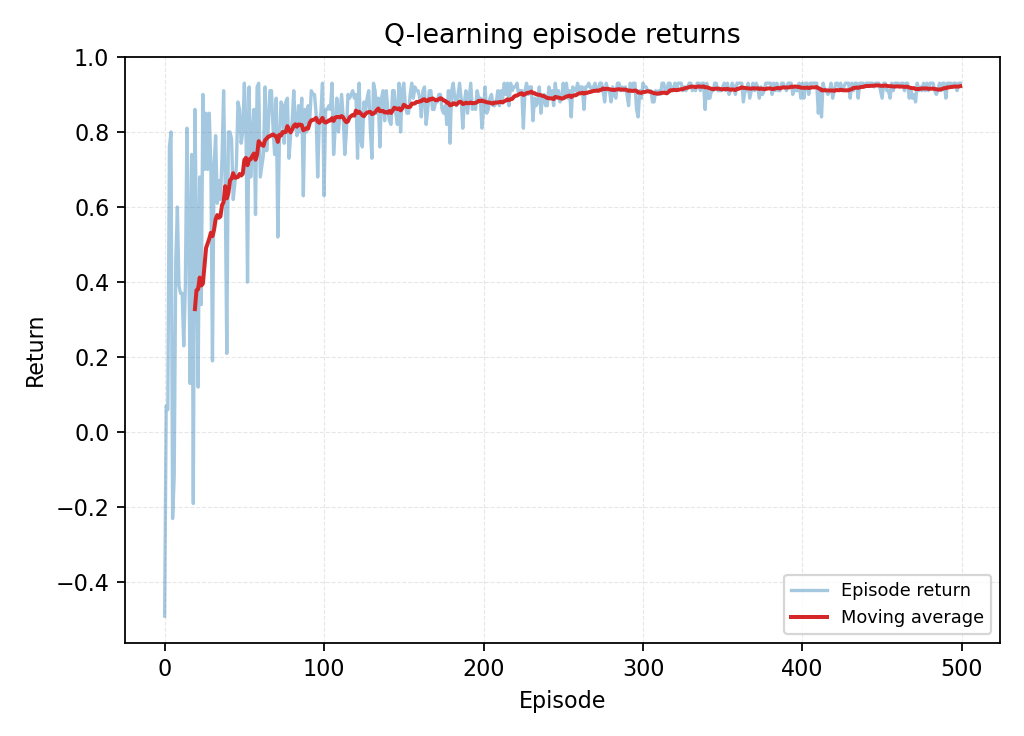
\includegraphics[width=0.8\linewidth]{q_learning_returns.png}
  \caption{Q-learning 回报曲线逐步逼近最优值}
  \label{fig:q_learning_returns_cn}
\end{figure}

\begin{figure}[H]
  \centering
  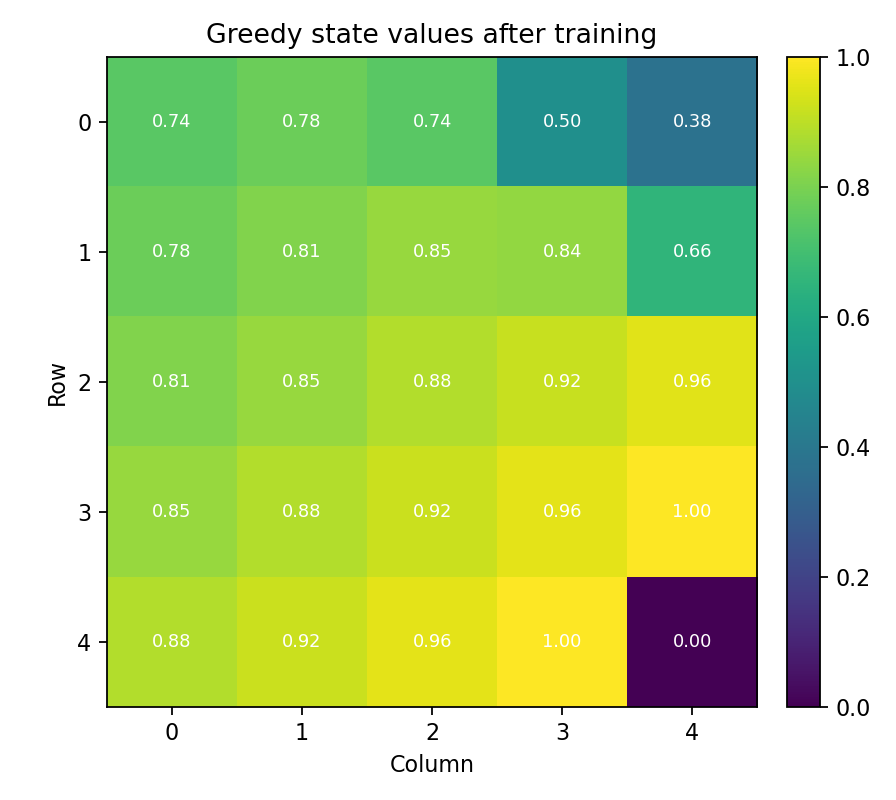
\includegraphics[width=0.82\linewidth]{q_learning_state_values.png}
  \caption{训练结束后的状态价值热力图,显示最短路径结构}
  \label{fig:q_learning_state_values_cn}
\end{figure}

\FloatBarrier
\section{总结}
Q-learning 通过时间差分和最大化操作估计最优动作价值。只要合理调节学习率、探索策略和奖励尺度,即可在众多离散环境中获得稳定的收敛效果。示例展示了回报的提升过程以及价值函数如何编码最优路径。

\end{document}